\begin{figure}[]
     \centering
     \def\w{0.45\linewidth}
     \begin{subfigure}{\w}
         \centering
         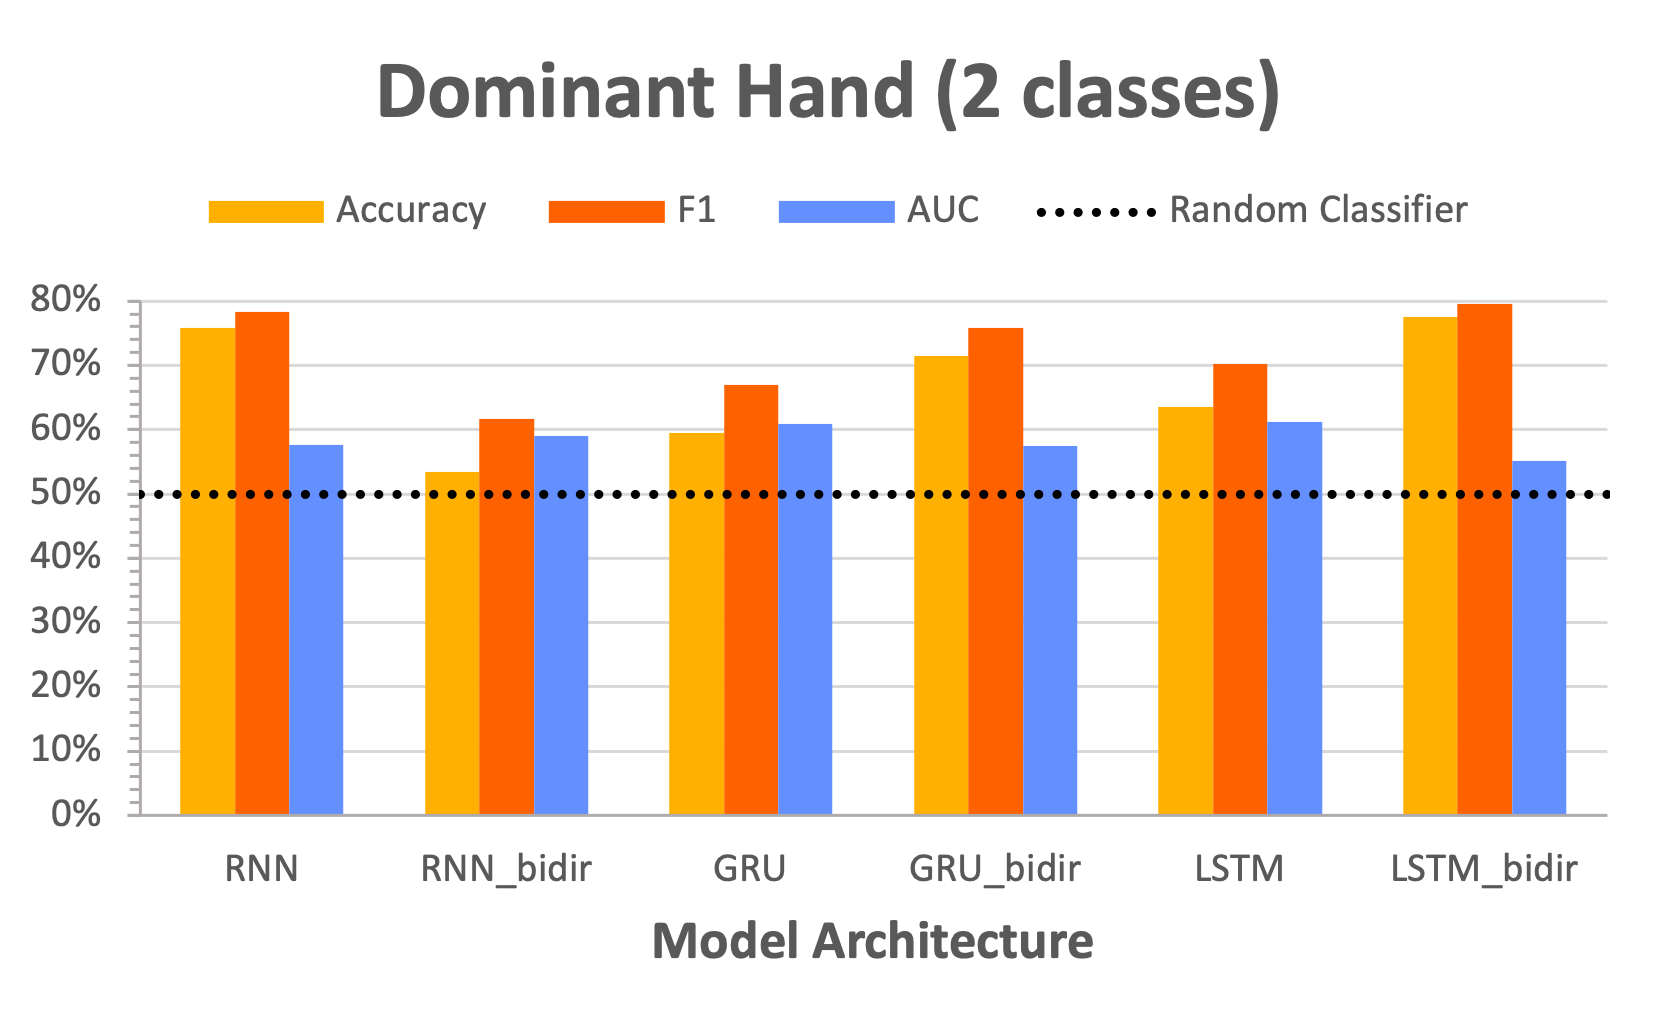
\includegraphics[width=\textwidth]{plots/model_dom.png}
         \caption{Layer type}
         \label{fig:models_dom}
     \end{subfigure}
     \hfill
     \begin{subfigure}{\w}
         \centering
         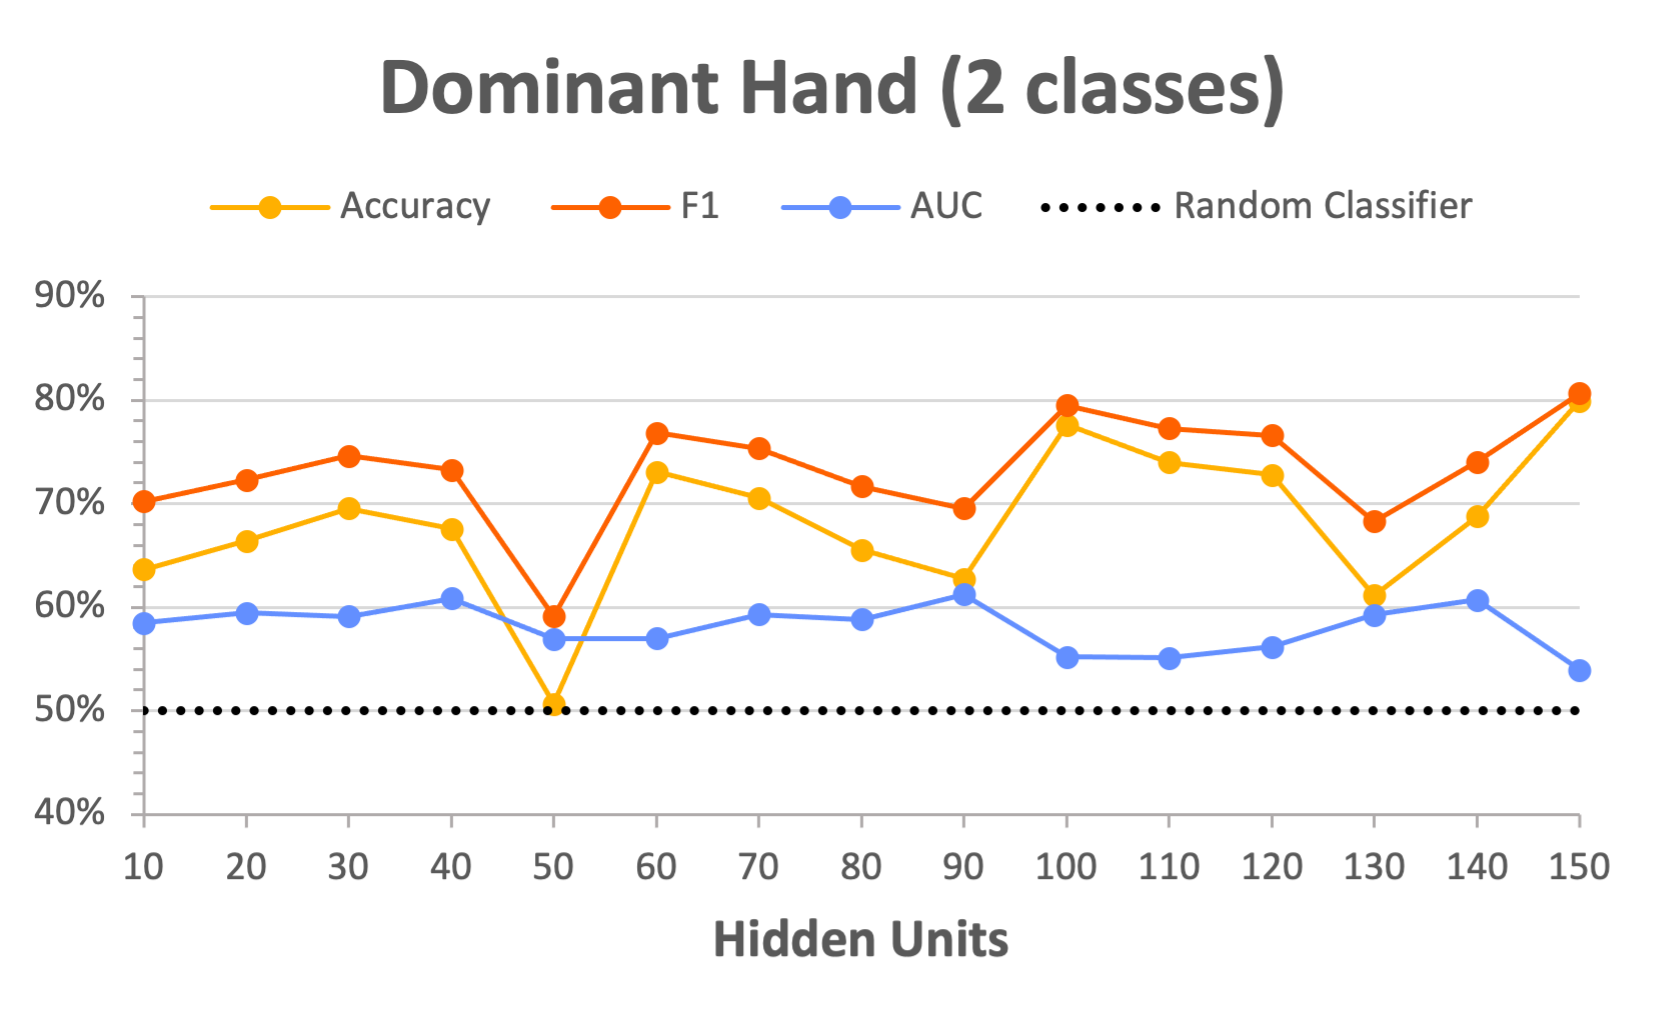
\includegraphics[width=\textwidth]{plots/units_dom.png}
         \caption{Hidden Units}
         \label{fig:units_dom}
     \end{subfigure}\\
     \begin{subfigure}{\w}
         \centering
         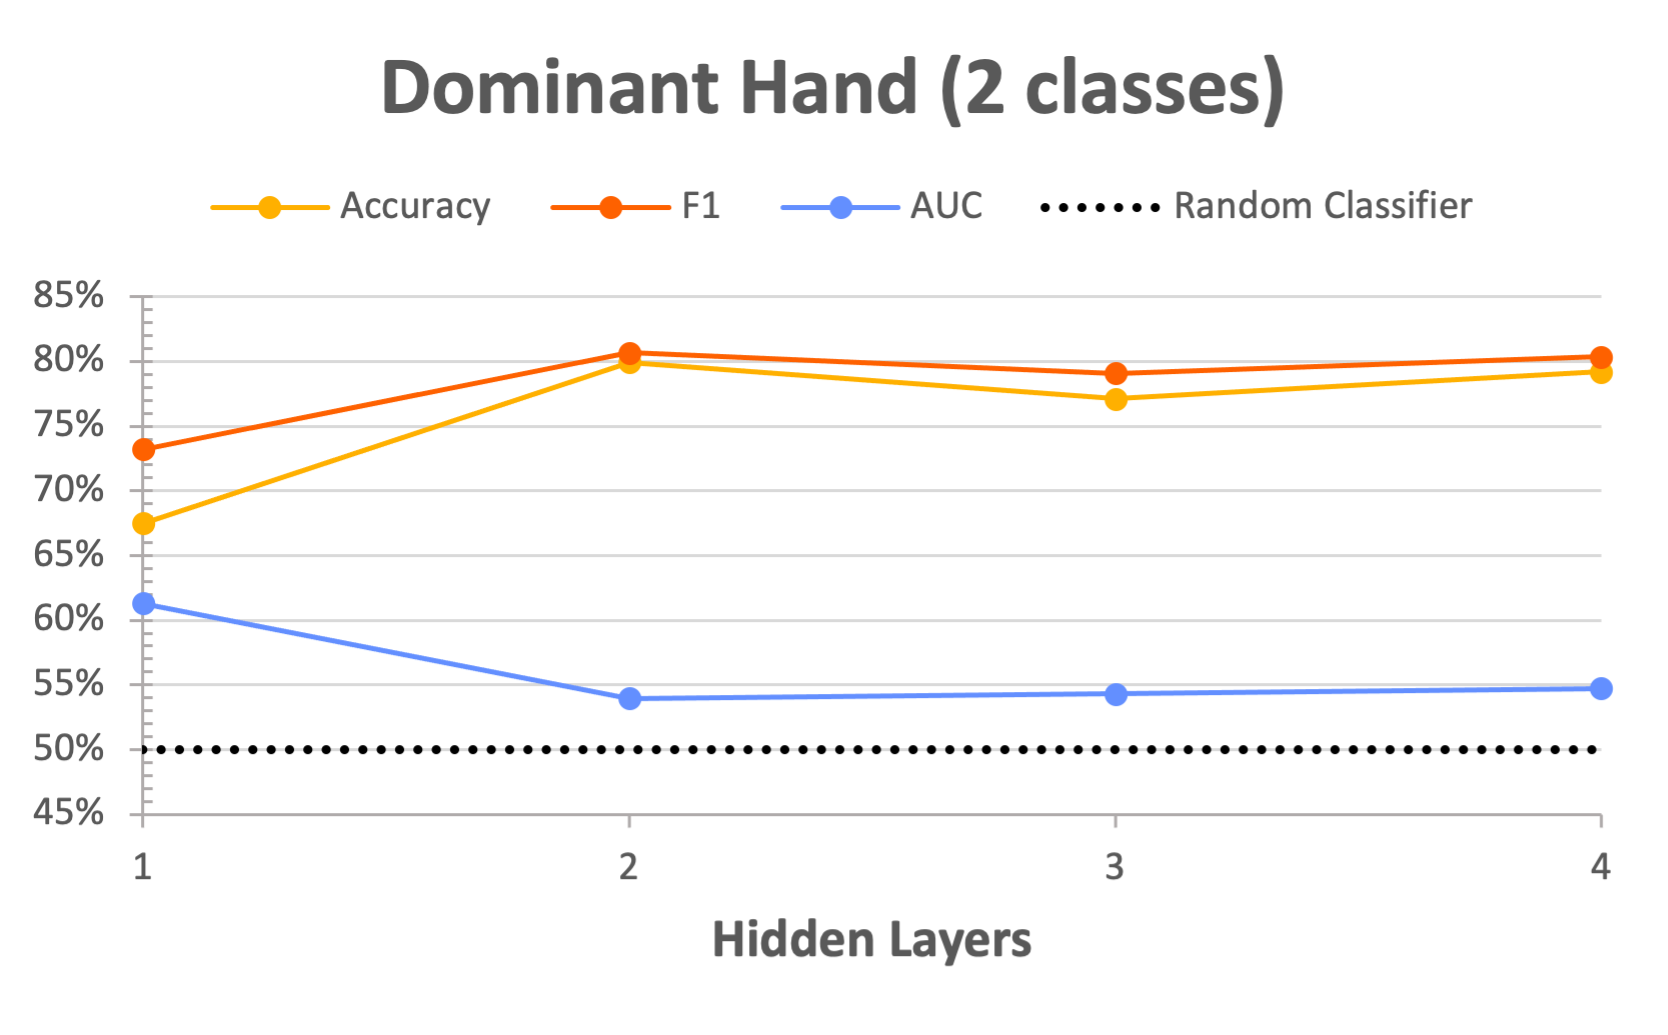
\includegraphics[width=\textwidth]{plots/layers_dom.png}
         \caption{Hidden Layers}
         \label{fig:layers_dom}
     \end{subfigure}
     \hfill
     \begin{subfigure}{\w}
         \centering
         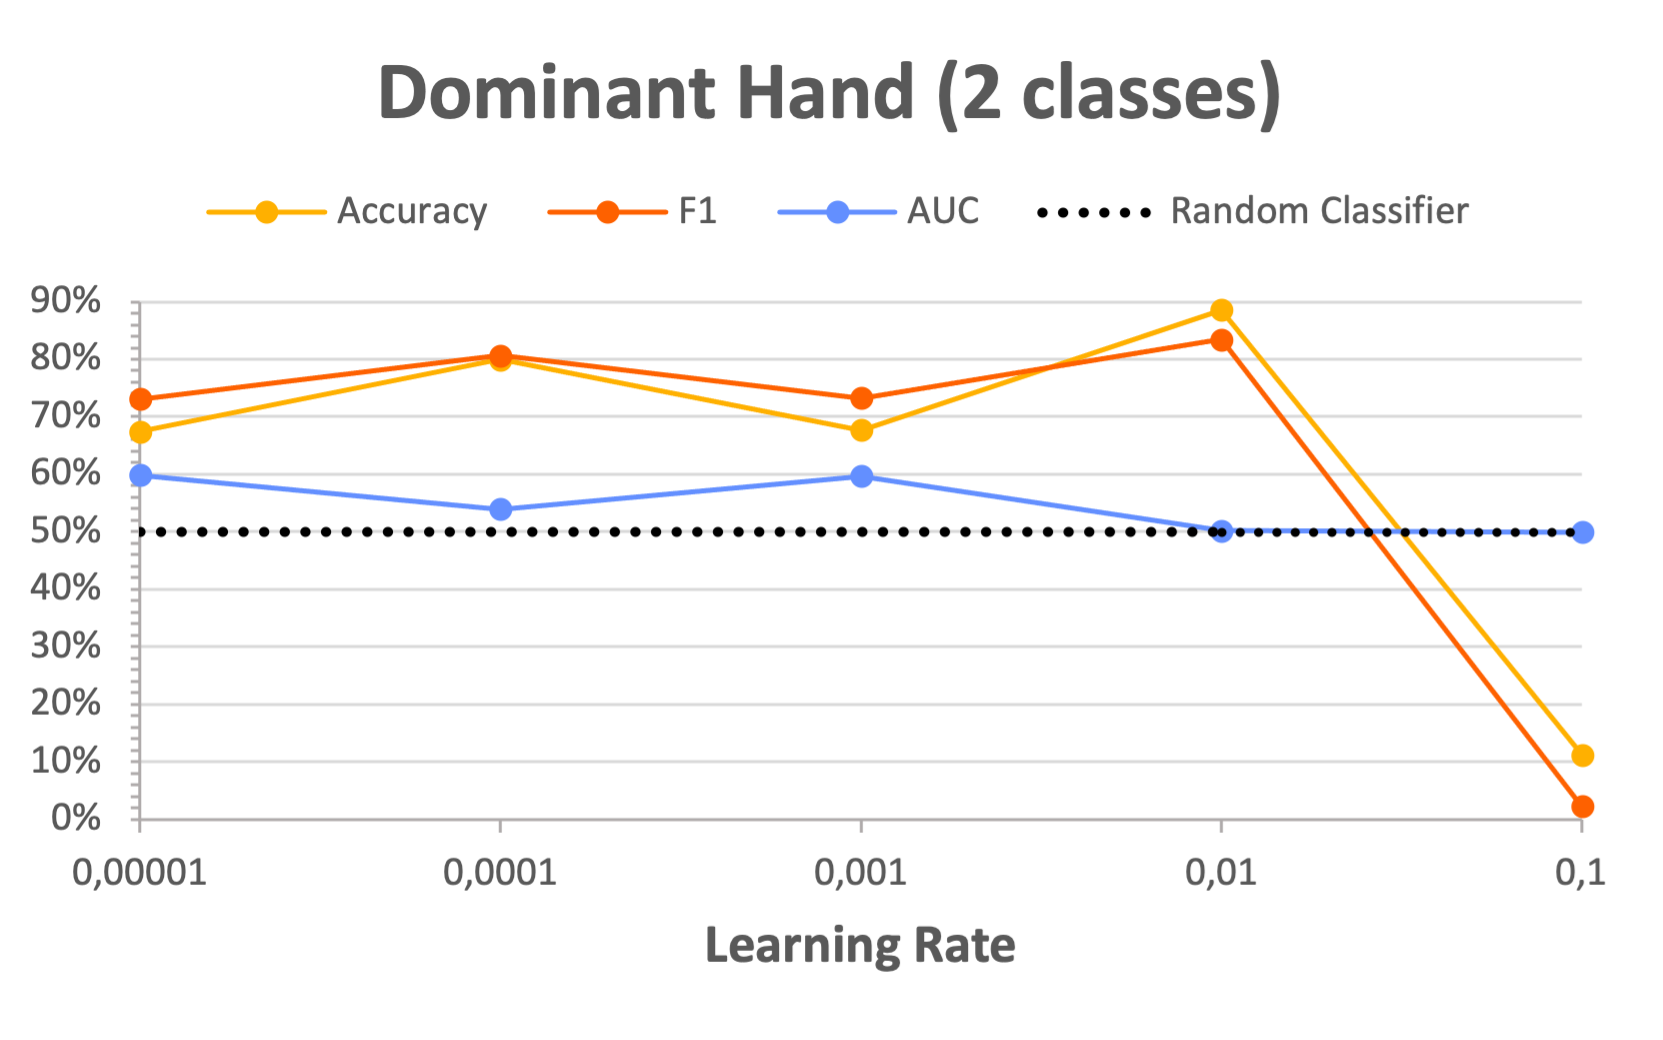
\includegraphics[width=\textwidth]{plots/lr_dom.png}
         \caption{Learning Rate}
         \label{fig:lr_dom}
     \end{subfigure}

    \caption{Predicting the user's dominant hand from swiped words trajectories.}
    \label{fig:dom}
\end{figure}
